\section{Design Overview}
In this section, we illustrate how the next three sections organized. 
In Section~\ref{sec_patterns}, we identify three typical OpenCL patterns, which are well understood by the conventional OpenCL programmer with GPUs.
In Section~\ref{sec_execution_models}, we generally analyze the characteristics of four OpenCL execution models, which takes into account the go-beyond OpenCL features enabled on FPGAs.
In Section~\ref{sec_bridge_gap}, we explicitly bridge the gap between OpenCL patterns and execution models on FPGAs. Choosing the right execution model determines the performance upper bound of the interested OpenCL application can reach. %can deliver an order of magnitude performance difference. 
\vspace{-1ex}
\section{Three OpenCL Patterns}%: Issue and Potential
\label{sec_patterns}
%The conventional OpenCL is originally designed for GPUs which have super powerful memory subsystem, 
When migrating conventional OpenCL programs, which is originally designed for GPUs, we identify three OpenCL patterns which can be significantly improved: atomic operation, multi-pass scheme and communication approach. In the following, we analyze the issue and potential optimization direction of each pattern on FPGAs.

\vspace{-1ex}
\subsection{Atomic Operation (AO)}
For NDRange OpenCL, the atomic operation is required to guarantee the consistence of OpenCL kernel, when multiple work items try to update the same memory location~\cite{opencl_spec, atomic_fpga16}. It provides the improved programmability that GPU programmers nowadays leverage, since the hardware for the atomic operation has greatly improved in recent GPU generations (e.g., NVIDIA Kepler, Maxwell, Pascal).
Take as an example the simplified histogram, whose main body is illustrated in Listing~\ref{list_atomic_histo}. %, style=base

%\begin{lstlisting}[caption={Atomic-based histogram},label={list_atomic_histo},captionpos=b]
\begin{lstlisting}[caption={Atomic-based histogram},label={list_atomic_histo},captionpos=b]
int tid = get_global_id(0);//global work item
int d   = data[tid];       //fetch the data from memory
int h_d = hash(d);         //compute the hash index
atomic_add(&@hist@[h_d],1);  //atomically add to hist
\end{lstlisting}

%@jiang, add one example here.

{\bf Issues on FPGAs. }We have identified three issues regarding atomic operation on FPGAs. First, the mechanism of atomic operation is relatively complex, so massive FPGA resources are required to implement it, leading to a noticeable resource overhead on FPGAs. %and then this issue on FPGAs is much worse on ASICs. 
Second, with atomic operation in our OpenCL kernel, all the memory transactions, including both atomic and normal memory transactions, have to enter the atomic module to guarantee the correct execution, as atomic and normal memory transactions from OpenCL kernel can reference the same memory location. Therefore, each memory transaction has a longer memory access latency, leading to potentially lower memory bandwidth.  
Third, the frequency of OpenCL kernel with atomic operation is slightly lower than that without atomic operation, leading to lower performance. We conclude that the atomic operation is not able to fit well on FPGAs.  % has severe performance issue \jgl{Every access goes through the atomic path even though it is clear that there are no atomic accesses to certain arrays? This is weird, but reminds me that something similar happened in old AMD GPUs}

{\bf Potential on FPGAs. }In order to achieve good performance of OpenCL kernel on FPGAs, one potential direction is to get rid of atomic operation. Fortunately, Intel OpenCL SDK~\cite{altera_optimization} supports a new execution model: SWI kernel. Essentially, it contains only one work item during the kernel execution, so there is no conflict from multiple work items, indicating that no atomic operation is required. Instead, it exploits the pipelined parallelism, not the thread-level parallelism which is widely exploited by GPUs. The previous histogram application is converted into the SWI kernel as shown in Listing~\ref{list_swi_histo}. 

\begin{lstlisting}[caption={SWI-based histogram},label={list_swi_histo},captionpos=b]
for (t=0; t<size; t++) { //for loop instead of work item
  int d   = data[t];     //fetch the data from memory
  int h_d = hash(d);     //compute the hash index
  @hist@[h_d] += 1;        //accumulate to hist
}
\end{lstlisting}


\vspace{-1ex}
\subsection{Multi-Pass Scheme (MPS)}
The multi-pass scheme is widely adopted to leverage a massive amount of cores in CPUs/GPUs to accelerate parallel algorithm, e.g., database operators~\cite{query_gpu_tods09, omnidb_vldb13, query_openCL_fpga_fpl16}. Besides, it can also improve the cache locality on GPUs, e.g., gather/scatter~\cite{gather_scatter_sc07}, so as to increase the overall parallelism at the cost of more memory traffic. Take the simplified parallel prefix sum~\cite{scan_gpu_nvidia07} as an example, we perform the prefix sum on the input array \emph{in} of size \emph{N} and store the output in the array \emph{out}, as illustrated in Listing~\ref{list_parallel_scan}. In Step 1, B work groups (WGs) executes concurrently, each WG performs the prefix sum (kernel \emph{prefix\_sum\_wg}) on its own part of data of starting address \emph{in[N*b/B]} and of length \emph{N/B}. Meanwhile, each WG stores its local sum to \emph{local\_sum}. In Step 2, we employ one WG to compute the prefix sum on \emph{local\_sum} and store to \emph{pre\_bsum}. In Step 3, each WG adds the scalar value \emph{pre\_bsum} to the vector and then produces the final prefix sum. 

% illustrates the B-work-group parallelism. 
\begin{lstlisting}[caption={MPS-based prefix sum},label={list_parallel_scan},captionpos=b]
//Step 1: each WG computes the prefix sum on its own data
#progama parallel in B work groups
for (b = 0, b < B, b++) { 
  local_sum[b] = prefix_sum_wg(@out@[N*b/B],@in@[N*b/B],N/B);
}

//Step 2: one WG computes the prefix sum on "local_sum"
prefix_sum_wg(pre_bsum, local_sum, B);

//Step 3: out@[b*N/B] += pre_bsum[b]
#progama parallel in B work groups
for (b = 0, b < B, b++) {
  vec_add(@out@[b*N/B], @out@[b*N/B], pre_bsum[b], N/B);
}
\end{lstlisting}
%Therefore, the multi-pass scheme, which heavily relies on high memory bandwidth, can still achieve better performance on GPUs than on CPUs, even though it requires multiple times more memory traffic than the original sequential counterpart which may run on a single CPU core. 
%requires multiple passes~\cite{query_gpu_tods09} to finish the computation task, e.g., database scan. In other words,

{\bf Issues on FPGAs. }We observe that the inevitable requirement for the widespread adoption of multi-pass scheme is powerful memory subsystem, as it always requires multiple times more memory traffic to realize the algorithm. It works pretty well on GPUs, whose memory bandwidth is almost an order of magnitude larger than the same-generation CPU or FPGA. For example, the memory bandwidth of Nvidia Tesla P100 GPU is able to reach 732GB/s, while Intel Skylake i9-7980XE CPU has the memory bandwidth of 85GB/s and Xilinx UltraScale+ FPGA board has 48GB/s. We can predict that the multi-pass scheme, whose success heavily relies on high memory bandwidth, would be less popular on FPGAs than on GPUs, since the memory bandwidth of FPGAs is relatively low, e.g., 18GB/s on our tested FPGA board. Therefore, it suffers from its severe performance issue, especially for the memory-bound OpenCL kernel, even though the FPGA can provide massive thread-level parallelism in terms of pipelined parallelism. 

{\bf Potential on FPGAs. } Since Intel OpenCL SDK for FPGAs supports the new single work-item kernel, the OpenCL kernel is allowed to be implemented in a single-pass approach, as illustrated in Listing~\ref{list_swi_scan}. %, without compromising any achievable pipeline parallelism 
Therefore, the memory traffic is reduced to a minimum level (i.e., accessing the array \emph{in/out} once, not twice) just as the single-threaded implementation running on a single CPU core. 
%We can use single-work item execution model: multi-pass approach to approach. %It means that the memory traffic 
\begin{lstlisting}[caption={SWI-based prefix sum},label={list_swi_scan},captionpos=b]
out[0] = 0;
for (t=1; t<n; t++) { //for loop instead of work item
  @out@[t] = @out@[t-1] + @in@[t]; //dependency in out
}
\end{lstlisting}



\vspace{-1ex}
\subsection{Kernel-to-Kernel Communication (KKC)}
On GPUs, the typical communication approach between producer/consumer kernels is done via global memory. In particular, after the producer kernel writes the data to the global memory, the consumer kernel reads the data from global memory, as illustrated in Figure~\ref{fig_without_channel}. It is a common communication approach to exchange information among Stream Processors (SPs) in GPUs, as there is no physical communication path between any two SPs. This communication approach works well on GPUs since GPUs can execute each kernel relatively fast due to its massive thread-level parallelism and powerful memory subsystem. Suppose each OpenCL kernel is fully optimized, the overall performance of producer/consumer kernels is maximized. %Even though more memory traffic is required to 
This communication approaches widely used in accelerating various applications, e.g., database~\cite{query_gpu_tods09, omnidb_vldb13}. 

{\bf Issue on FPGAs. }The memory bandwidth is relatively low on FPGAs, e.g., 18GB/s on our FPGA board, the communication via external memory can be expensive, compared with that on GPUs. 

{\bf Potential on FPGAs. }We can use OpenCL channel via which the producer kernel can directly send data to the consumer kernel at the register level (i.e., FIFO), without any memory traffic involved between the producer and consumer kernels, as illustrated in Figure~\ref{fig_with_channel}. Besides, both kernels, each of which has the dedicated hardware resources to implement, execute concurrently, so not only intra-kernel parallelism (i.e., pipelined) is exploited, but also inter-kernel parallelism (i.e., multiple kernels).  
\begin{figure}
	\centering
	%\hfill
	\subfloat[Without channel]{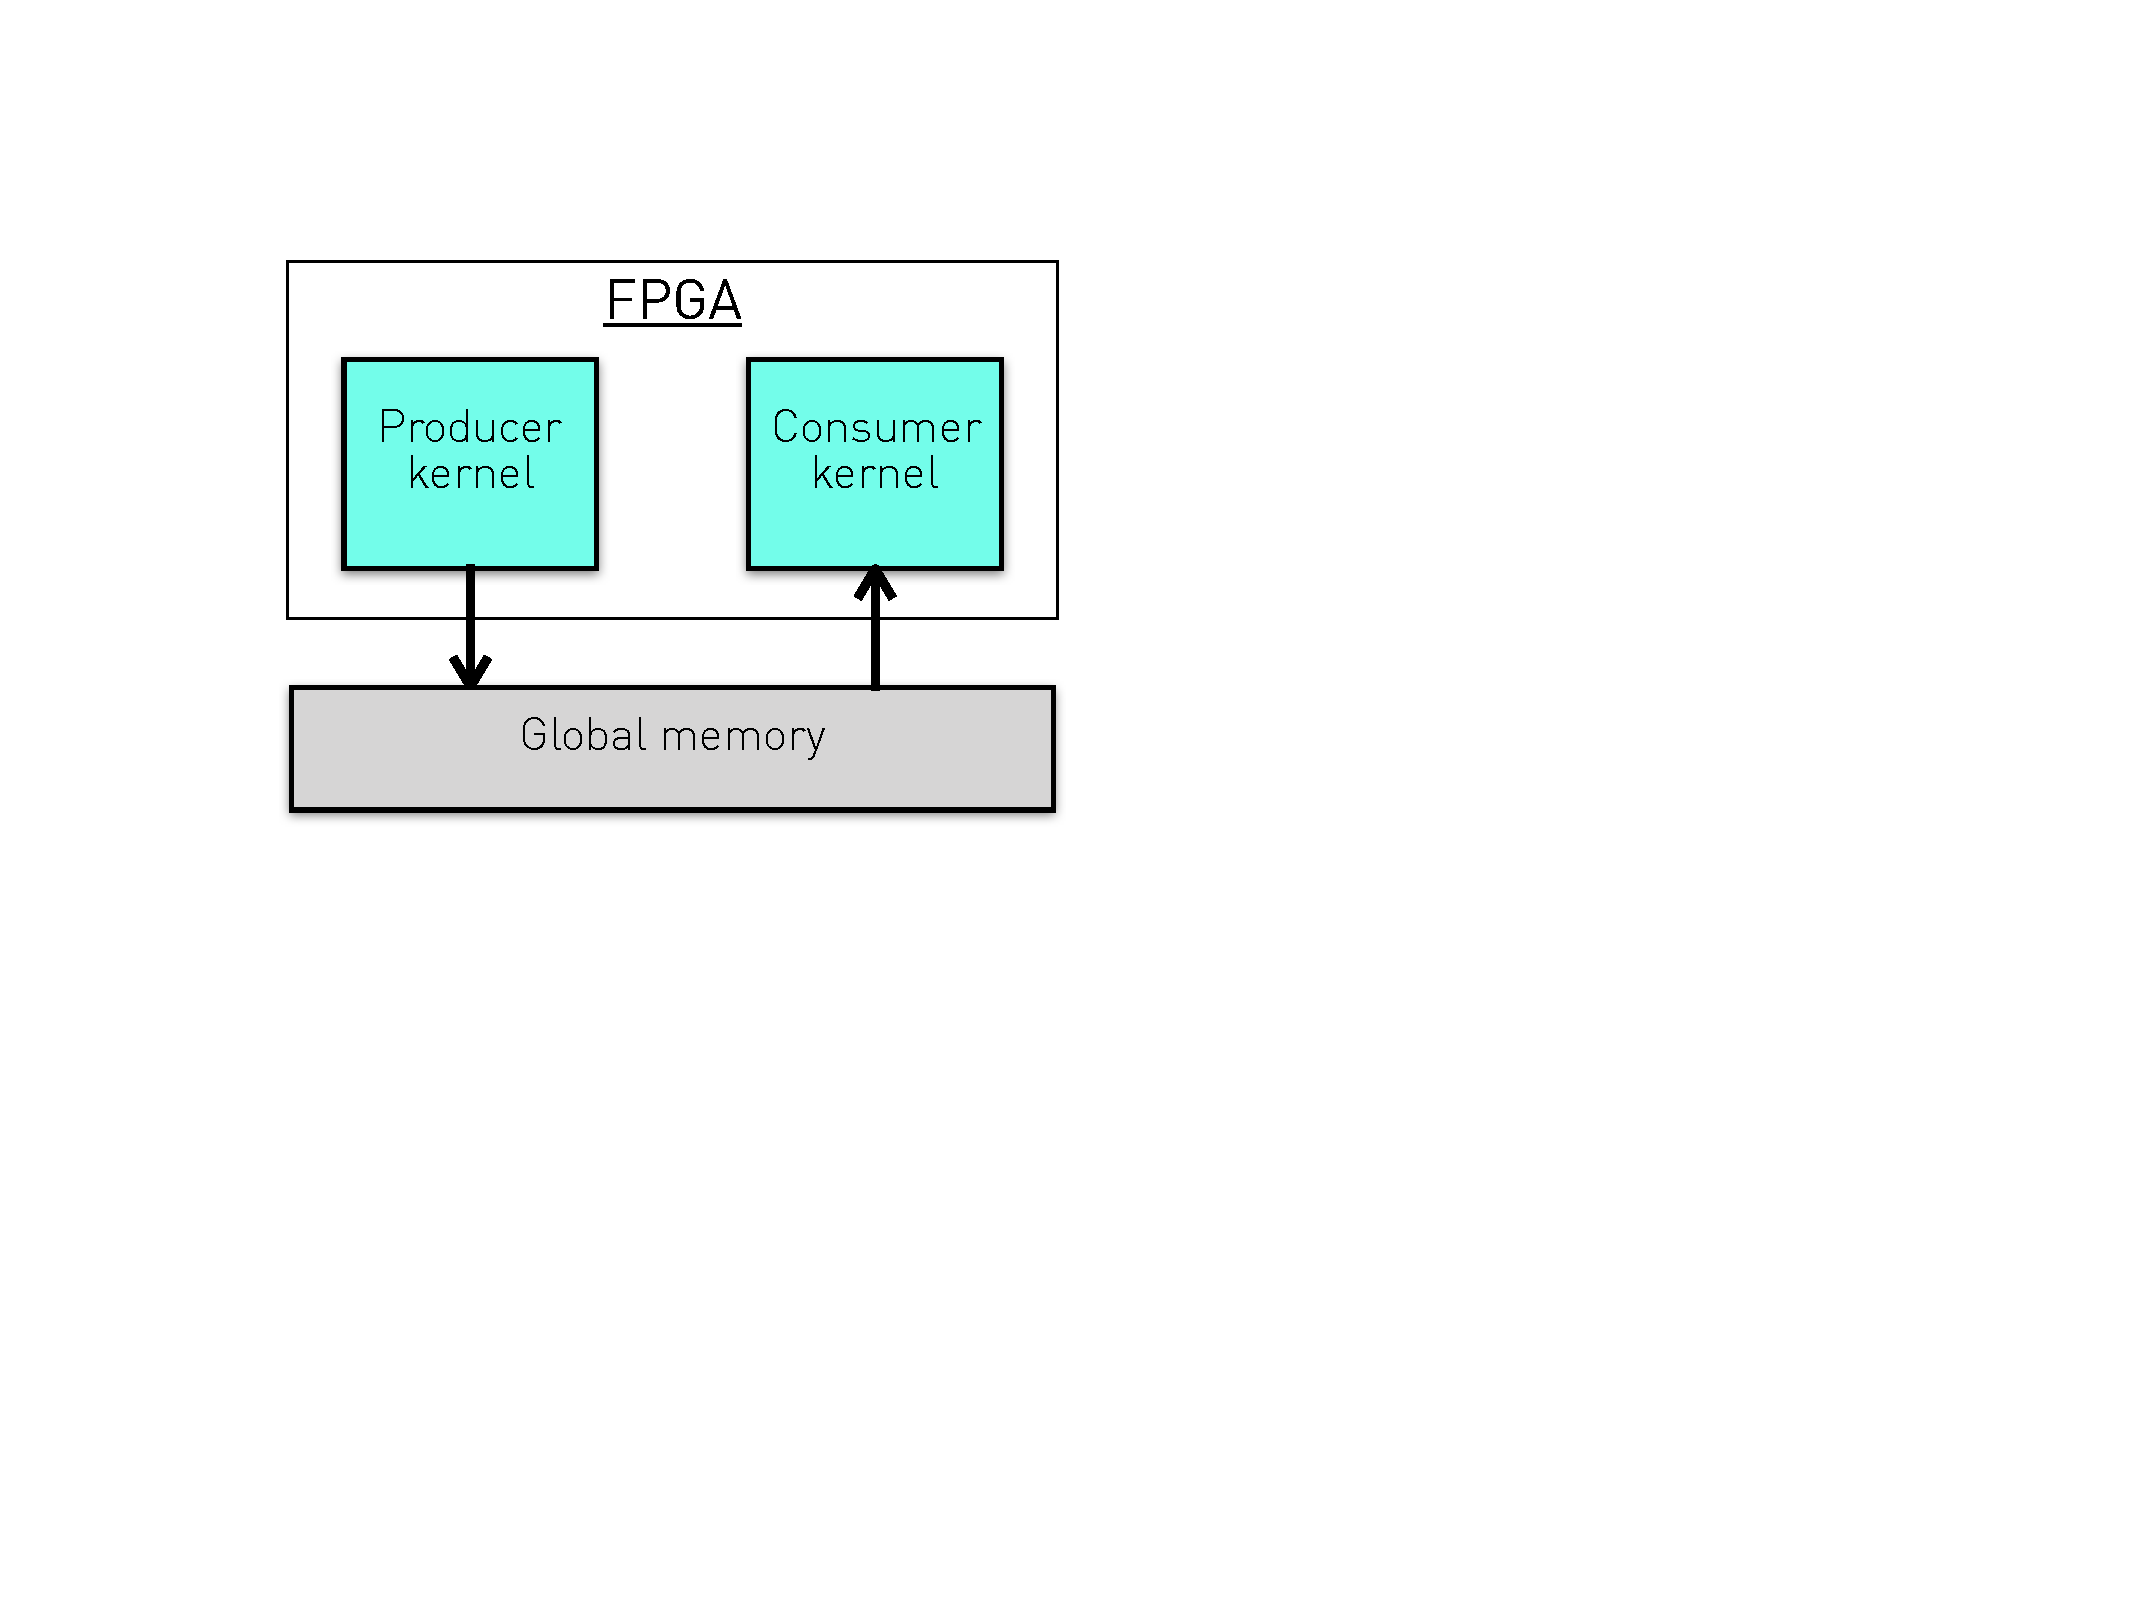
\includegraphics[width=1.415in]{without_channel1.pdf} 
		\label{fig_without_channel}} 
	\subfloat[With channel]{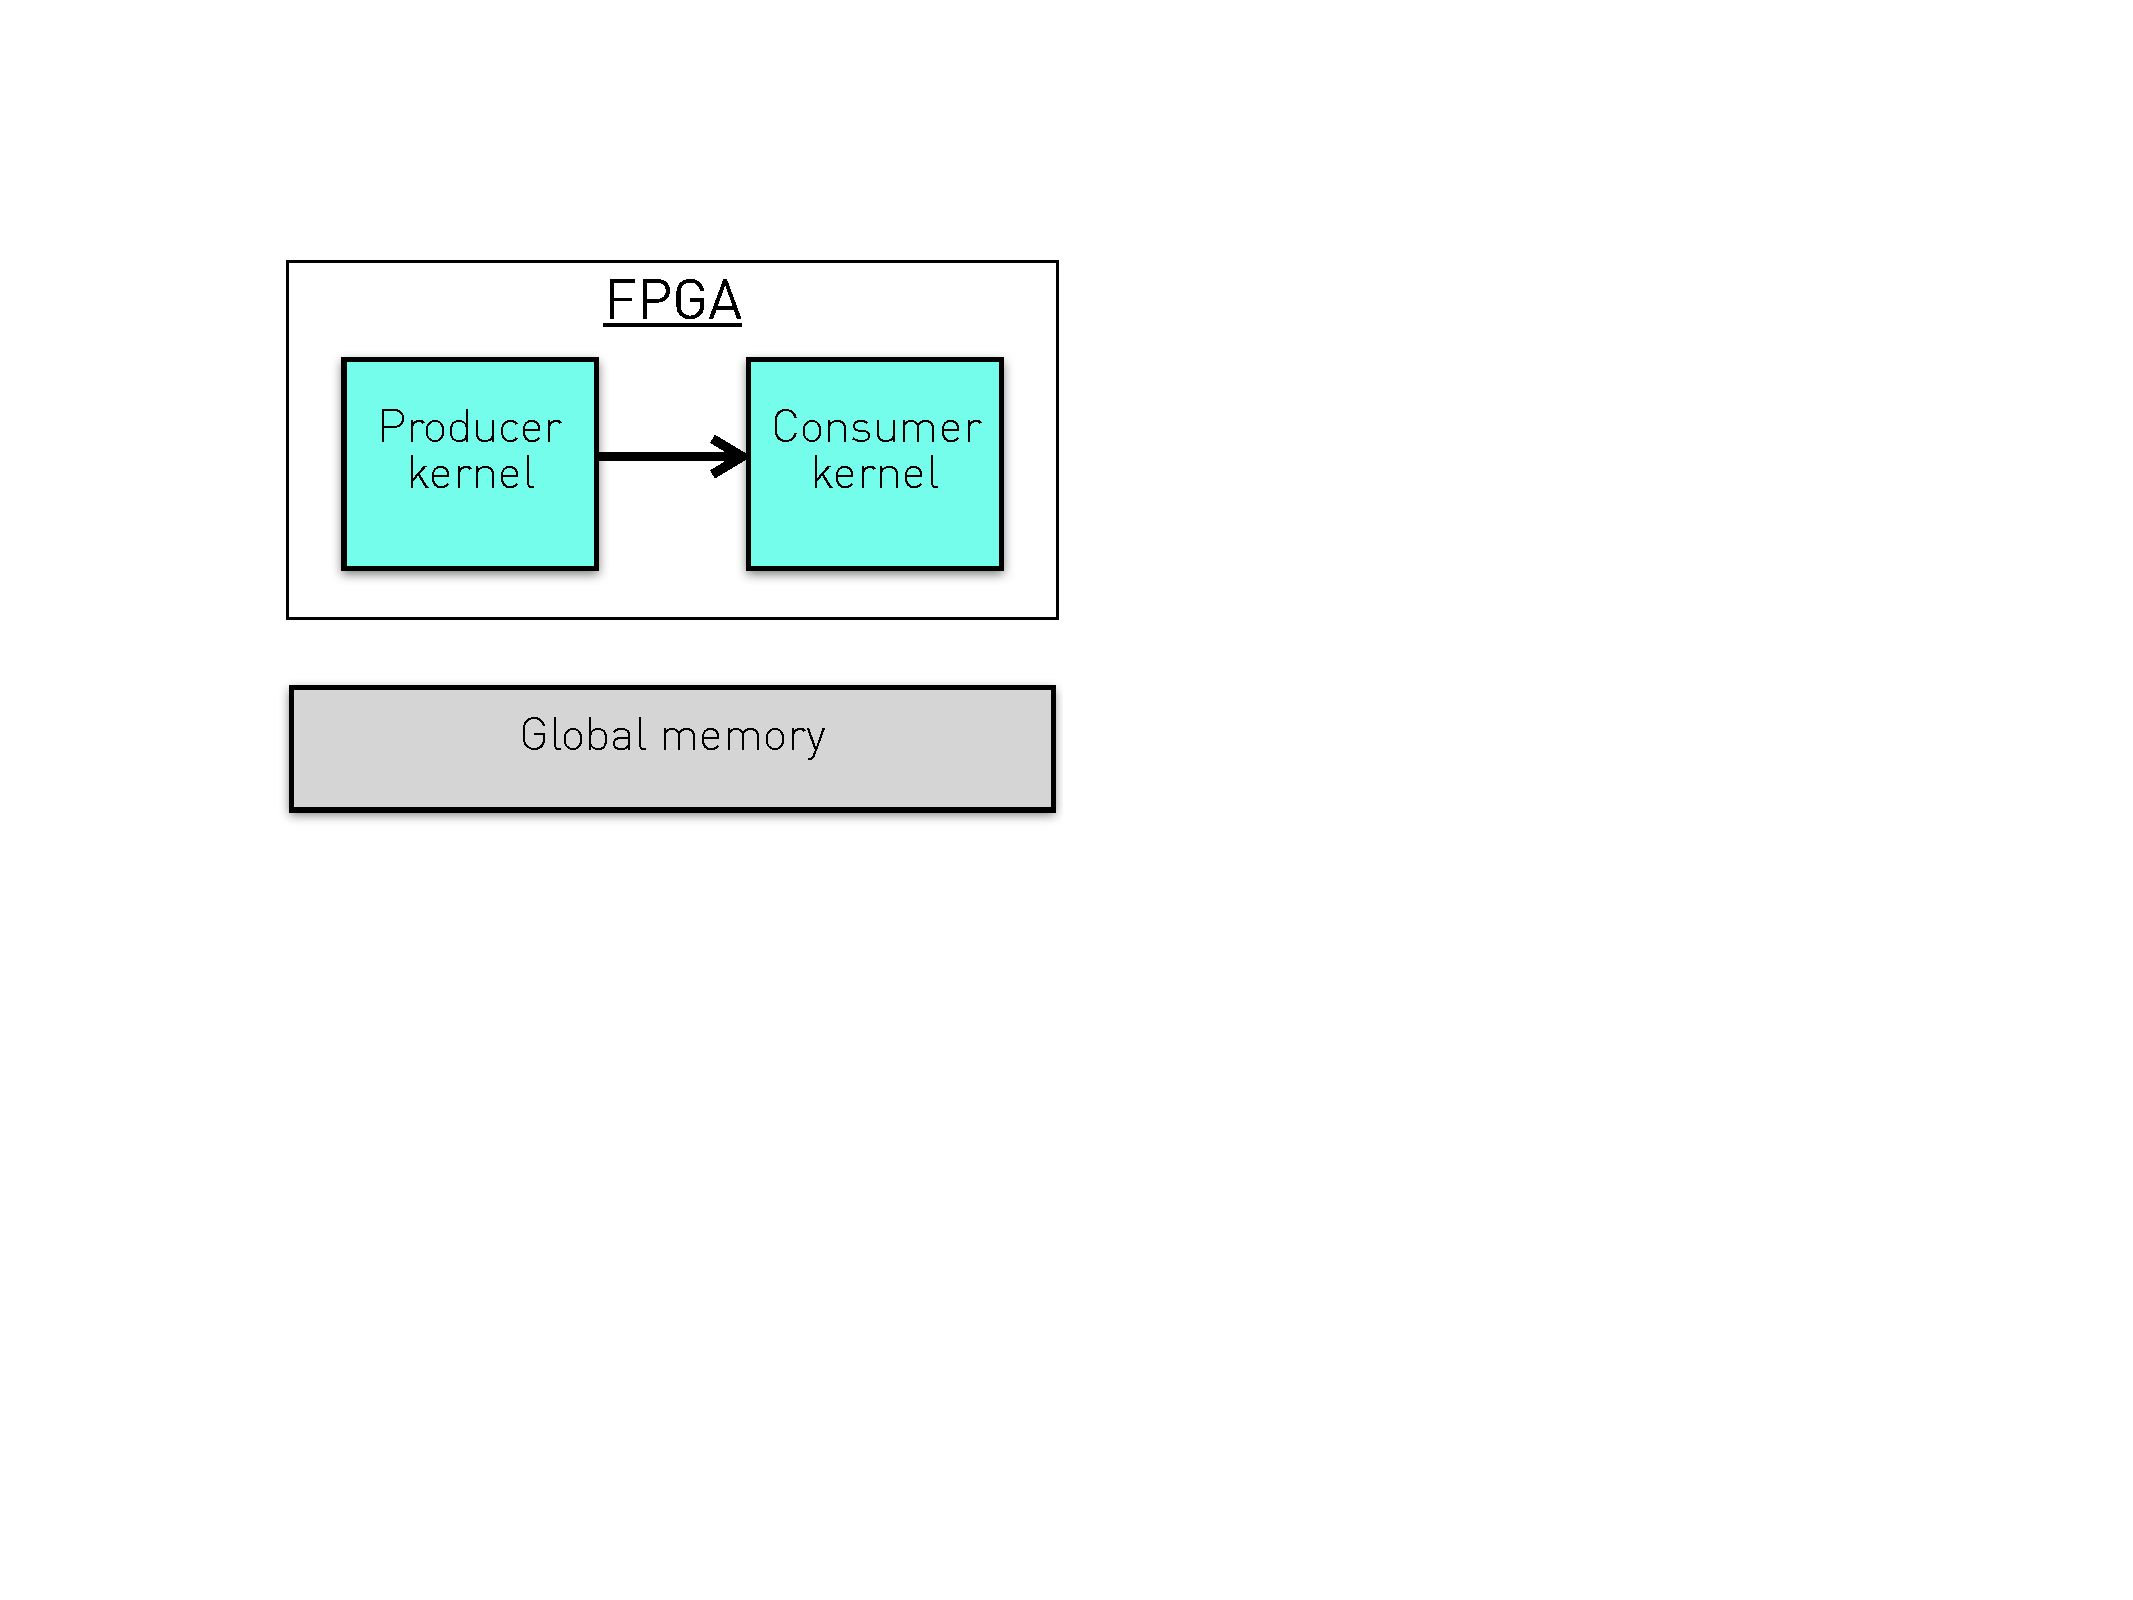
\includegraphics[width=1.4in]{with_channel.pdf} 
		\label{fig_with_channel}} % \caption{}
	\vspace{-2ex}	
	\caption{Kernel-to-kernel communication.} %: Hogwild and ModelAverage$\lambda$ is $1/2^{10}$ (``with RAW"), or $1/2^{13}$ (``without RAW"). 
	\label{fig_kkc} 
	\vspace{-2ex}
\end{figure}  



%\subsection{Dependency}
%For compute-bound applications, which can be benefited from exploring more parallelism among work items. 

\vspace{-1ex}
\section{Four OpenCL Execution Models}
\label{sec_execution_models}
%Since the architecture of FPGAs is significantly different from that of GPUs, we need to revisit the OpenCL execution models on FPGAs. with the proposed aspects in mind, 
Enabled by two go-beyond features of OpenCL on FPGAs, we identify four execution models in the context of OpenCL kernel on FPGAs. In this section, we generally analyze each execution model, in terms of programmability, computing parallelism and memory traffic. The comparison is highlighted in Table~\ref{t_comparison}.%The detailed 
%{NDRange vs. single work-item}
%{single-kernel vs. multiple kernels connected by OpenCL channel }

\begin{table} %[!hbp]
	\centering
	%\begin{spacing}{0.3}
		\begin{scriptsize}
	\begin{tabular}{|c|c|c|c|c|}
		\hline
		  & NDRange & SWI & NDRange+Channel & SWI+Channel \\
		\hline
Programmability & Moderate & High & Low & Low \\
		\hline
Computing Parallelism & Moderate & Low & High & High \\
		\hline
Memory Traffic & High & Low & Moderate & Low \\
		\hline		
	\end{tabular}
		\end{scriptsize}
	%\end{spacing}
		\caption{General comparison of four execution models}
	%\vspace{-1ex}
	\label{t_comparison}
	\vspace{-6ex}
\end{table}


\vspace{-1ex}
\subsection{NDRange}
The NDRange execution model directly employs the NDRange kernel, which is the conventional OpenCL programming mode and which is widely adopted in GPU programming. It explores a massive thread-level parallelism. The optimization methods which are used by GPUs can also apply to FPGAs, e.g., shared memory. %, memory coalescing.

{\bf Programmability. }The OpenCL programmer needs to be aware of the activity of each thread to guarantee the correct execution. Therefore, it is much more difficult than the traditional sequential programming language, e.g., C. However, there is plenty of tutorial on how to program NDRange kernel, especially for GPUs, so the programmability of NDRange execution model is moderate.

{\bf Computing Parallelism. }NDRange kernel relies on massive amount of work items to explore the parallelism from the specialized hardware generated from the NDRange kernel. Therefore, we conclude that it can achieve a high computing parallelism.  

{\bf Memory Traffic. }NDRange kernel employs the multi-pass scheme to implement the parallel algorithm, leading to potentially multiple times more memory traffic. We conclude that the requirement of memory traffic is high. 
%{\bf Cons. }It may not achieve good performance on FPGAs, whose architecture is significantly different from GPUs. Suppose it works well on FPGAs, it also works well on GPUs.
%{\bf Scope. }Without any above three issues. 

\vspace{-1ex}
\subsection{Single Work-item (SWI)}
\label{subsec_swi} 
The SWI execution model directly employs the SWI kernel, which follows a sequential programming model. %In the single work-item execution pattern, the parallelism is implicit, and the OpenCL SDK will instead determine pipelined parallelism at the compilation time based on the dependency. 
%Only one work-item is alive during the execution. 


{\bf Programmability. }Programming with SWI kernel is just like C programming. Therefore, it is relatively easy to program. We conclude that the programmability of SWI kernel is high.

{\bf Computing Parallelism. }SWI kernel relies on the off-line compiler to explore the parallelism. In order to guarantee the consistence, the compiler is always conservative, leading to a low computing parallelism.  

{\bf Memory Traffic. }SWI kernel can leverage a one-pass scheme (less memory traffic) to implement the parallel algorithm, instead of the multi-pass scheme (more memory traffic). We conclude that the SWI kernel requires a low memory traffic. 

%{\bf Pros. }Easy to write the program. 
%{\bf Cons. }
%{\bf Scope. }With Atomic or multi-pass, or both. But it works only for a simple OpenCL kernel, since it can only explore limited parallelism.

\vspace{-1ex}
\subsection{NDRange + Channel}
The NDRange + Channel execution model employs an OpenCL channel to connect two NDRange kernels such that the data communication between two kernels can be done via on-chip FIFO, rather than global memory. 

{\bf Programmability. }Besides the programming difficulty from NDRange kernel, we still need to be aware of the constraint from OpenCL Channel. In particular, the producer kernel has to produce the exact data flow which the consumer kernel wants. To make things worse, work items can execute out-of-order due to the different workload of each work item, leading to unexpected data flow from NDRange kernel. We conclude that the programmability of NDRange+Channel execution model is low.

{\bf Computing Parallelism. }
Besides the high computing parallelism from NDRange kernel, OpenCL channel allows producer/consumer kernels to execute concurrently, leading to a massive parallelism. Therefore, we conclude that it can achieve a high computing parallelism.  

{\bf Memory Traffic. }NDRange kernel requires a high memory traffic. The OpenCL channel can potentially reduce the memory traffic to a certain extent. We conclude that the NDRange + Channel execution model requires a moderate memory traffic. 

\begin{table}%[hbp]
	\centering
	\begin{scriptsize}
		\begin{tabular}{|c|c|c|c|c|c|}
			\hline
			AO & MPS & KKC & Direct prediction & Potential evolution \\		
			% the 3 pattern's name is too long
			\hline
			N & N & N & NDRange & NDRange  \\
			\hline
			Y & N & N & SWI  & SWI+Channel  \\
			\hline
			N & Y & N & SWI & SWI+Channel  \\
			\hline
			Y & Y & N & SWI & SWI+Channel  \\
			\hline
			N & N & Y & NDRange+Channel & NDRange+Channel \\
			\hline
			Y & N & Y & SWI+Channel & SWI+Channel  \\
			\hline
			N & Y & Y & SWI+Channel & SWI+Channel  \\
			\hline
			Y & Y & Y & SWI+Channel & SWI+Channel \\
			\hline
		\end{tabular}
	\end{scriptsize}
	\caption{Prediction rule}
	\label{t_pattern_to_model}
	\vspace{-6ex}
\end{table}


\vspace{-1ex}
\subsection{SWI + Channel }
The SWI + Channel execution model employs OpenCL channels to connect multiple SWI kernels such that multiple SWI kernels can work together to implement a parallel algorithm. The side effect of OpenCL channel is to relax the dependency of SWI kernel.  

{\bf Programmability. }SWI kernel has a high programmability, since its programming model is sequential. However, the OpenCL Channel incurs some constraint to guarantee the correct design. We conclude that the programmability of SWI+Channel execution model is moderate.

{\bf Computing Parallelism. }Even though the SWI kernel can achieve low computing parallelism, OpenCL channel can significantly increase the computing parallelism allows producer/consumer kernels to execute concurrently, leading to a massive parallelism. Therefore, we conclude that it can achieve a high computing parallelism.  

{\bf Memory Traffic. }SWI kernel requires a low memory traffic. The OpenCL channel might further reduce the memory traffic, so we conclude that the SWI + Channel execution model requires a low memory traffic. 



\vspace{-1ex}
\section{Bridge the Gap Between Patterns and Execution Models}%: Issue and Potential
\label{sec_bridge_gap}
In this section, we explicitly bridge the gap between three OpenCL patterns and four execution models. Typically, we can directly predict the right execution model based on three patterns (Subsection~\ref{subsec_direct_prediction}). However, there is an exception about SWI, which can only achieve low computing parallelism, indicating the further optimization potential. In particular, SWI can evolve to SWI+Channel to achieve high computing parallelism (Subsection~\ref{subsec_potential_prediction}).  

\vspace{-1ex}
\subsection{Direct Prediction}
\label{subsec_direct_prediction}
Based on whether the targeted OpenCL application has any patterns (i.e., the first three columns of Table~\ref{t_pattern_to_model}), we can directly predict the execution model, as illustrated in the ``Direct prediction" of Table~\ref{t_pattern_to_model}. Typically, the OpenCL application with AO and MPS can benefit from SWI kernel, while KKC can benefit from OpenCL channel.% indicate whether the 
\vspace{-1ex}
\subsection{Potential Evolution of SWI}
\label{subsec_potential_prediction}
In this subsection, we determine whether SWI should be evolved to SWI+Channel for higher computing parallelism, as shown in the column ``Potential evolution" of Table~\ref{t_pattern_to_model}. The evolution should satisfy two conditions. 

First, there are still enough FPGA resources remaining, as SWI+Channel, which instantiates more than one SWI kernels connected by Channel, requires significantly more FPGA resources to implement. 

Second, we present a simplified analytical model to predict the targeted SWI kernel is compute-bound or memory-bound. The evolution happens only when the SWI kernel is compute-bound. In particular, the computing time $T_{comp}$ is larger than memory time $T_{mem}$, as shown in Equation~\ref{E_overall_ineq}.
\begin{equation} \begin{scriptsize}
\label{E_overall_ineq}
\vspace{-0.5ex}
T_{comp} > T_{mem}
\vspace{-0.5ex}
\end{scriptsize} \end{equation}
The computing time $T_{comp}$ is evaluated as shown in Equation~\ref{E_comp}.
\begin{equation} \begin{scriptsize}
\label{E_comp}
\vspace{-0.5ex}
T_{comp} = \frac{LTR}{II}/\#Freq, 
\vspace{-0.5ex}
\end{scriptsize} \end{equation}
where the first part $LTR/II$ is the estimated number of cycles, equal to be the loop trip count $LTC$ divided by the initiation interval $II$. The second part $\#Freq$ is the frequency of the SWI kernel obtained from synthesis report. 
   
The memory time $T_{mem}$ is evaluated to be the number of memory traffic $MT$ divided by the memory bandwidth $\#MB$, as illustrated in Equation~\ref{E_mem}, where $\#MB$ is 18GB/s on our FPGA board.  
\begin{equation} \begin{scriptsize}
\label{E_mem}
\vspace{-0.5ex}
T_{mem} = \frac{MT}{\#MB} 
\vspace{-0.5ex}
\end{scriptsize} \end{equation}

%Direct connection + analytical model. 
